\documentclass[compress]{beamer}

\usepackage[spanish]{babel}
\usepackage[utf8]{inputenc}
\usepackage{amsfonts}
\usepackage{amsmath}
\usepackage{graphicx}
% \usepackage{subfigure}
\usepackage{fancyvrb}
%\usepackage{multicolumn}

\mode<presentation>
{
	\usetheme{Warsaw}
	\setbeamertemplate{headline}{}
	\setbeamertemplate{navigation symbols}{}
	\setbeamercovered{transparent}
	\useinnertheme{rectangles}
}
\setcounter{tocdepth}{1}

\title[Dreamster Workshop]{Dreamster Workshop @ RoboticsDay 2015}
\author[Robotics Day]
{
The Dreamster Community \\
Lucas, Lucía, Sebastián, Viviana, Martín, Gisela, Ignacio, Gary
}

\usepackage{default}

\begin{document}

\frame{\titlepage}

\section{Introducción}
\subsection{Objetivos}

\begin{frame}
 \frametitle{Bienvenidos}

\begin{columns}
\column{.5\textwidth}
\begin{center}
 
\includegraphics[width=\columnwidth]{./img/cdrfiuba.png}
\end{center}
\column{.5\textwidth}
\begin{center}
 
\includegraphics[width=\columnwidth]{./img/py.jpg}
\end{center}
\end{columns}

\end{frame}

\begin{frame}
 \frametitle{¿Qué vamos a hacer?}

\begin{center}
 \color{red}{\textbf{Limpiar un escritorio con un robot}}
\end{center}

\begin{block}{¿Cómo?}
\begin{itemize}
 \item Usando un Dreamster como base.
 \item Arduino para enseñarle a hacer cosas.
\end{itemize}
\end{block}

\begin{center}
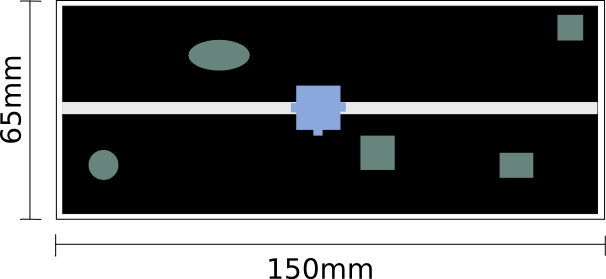
\includegraphics[width=0.8\textwidth]{./img/desk.png} 
\end{center}

\end{frame}
 
\begin{frame}
\begin{center}
\frametitle{¿Qué vamos a hacer?}

\includegraphics[width=0.6\textwidth]{./img/equipo.jpg}

\color{red}{\textbf{Trabajar en equipos}}
\end{center}
\begin{itemize}
 \item Cada equipo va a tener un robot
 \item Hoy y mañana preparamos los robots.
 \item El domingo hacemos una competencia.
\end{itemize}

\end{frame}

\subsection{Presentando el Arduino}

% Arduino fiscamente
\begin{frame}
 \frametitle{¿Qué es Arduino?}
\begin{block}{Arduino.cc dice:} 
\begin{itemize}
 \item Computadora que nos permite interactuar con el mundo real.
 \item Microcontrolador simple + entorno de desarrollo sencillo.
\end{itemize}
\end{block}
\begin{center}
 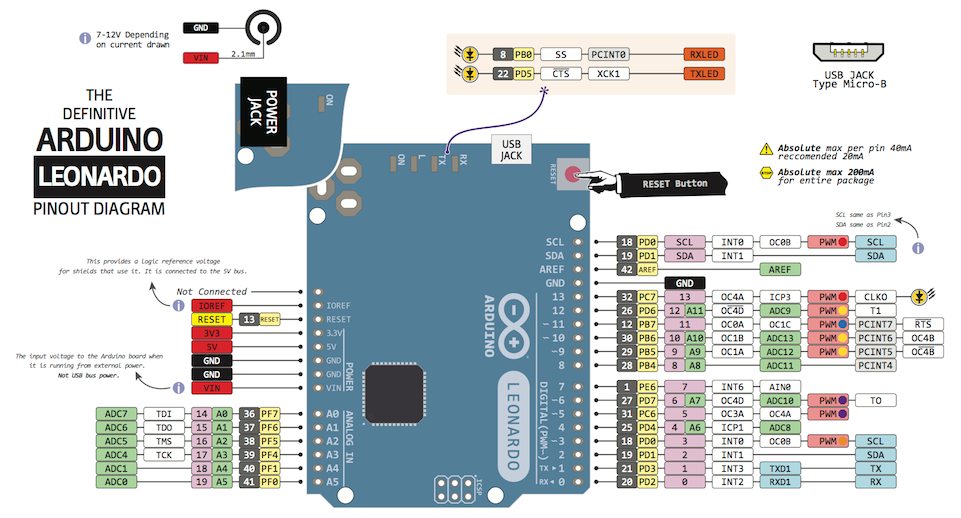
\includegraphics[height=0.6\textheight]{./img/arduino-leonardo-pinout.png}
\end{center}
\end{frame}

% Diferentes Arduinos
\begin{frame}
 \frametitle{¿Qué es Arduino?}
 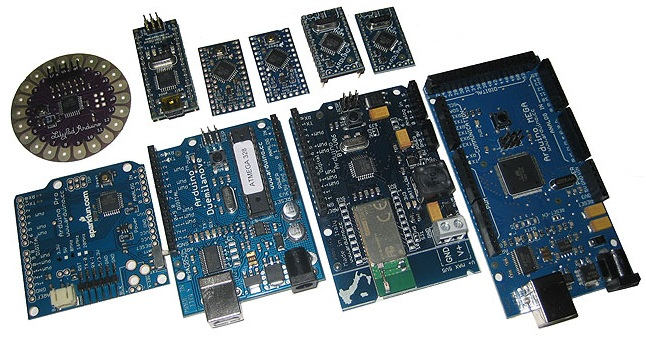
\includegraphics[width=\columnwidth]{./img/arduinos.jpg}
  \begin{itemize}
   \item Interfaces estándar.
   \item Diseños libres.
   \item Muchas formas y tamaños.
  \end{itemize}
\end{frame}

% Programando arduino
\begin{frame}
 \frametitle{¿Qué es Arduino?}
\begin{columns}
 \column{0.6\textwidth}
  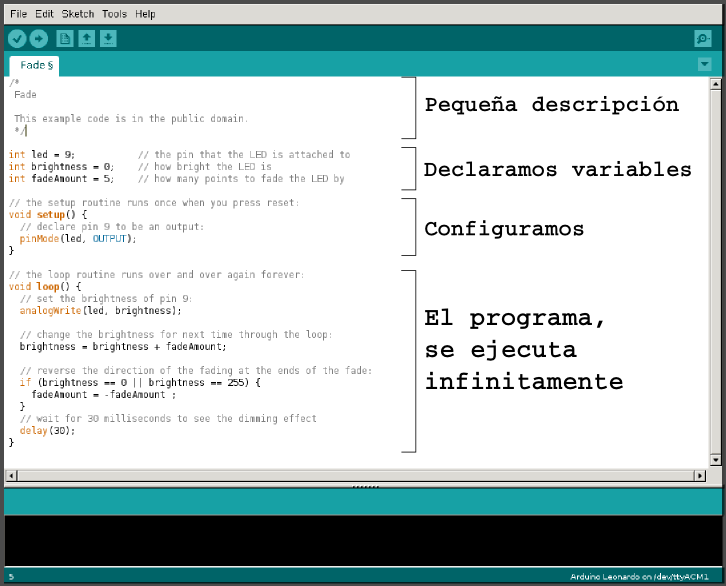
\includegraphics[width=\columnwidth]{./img/arduino-ide-text.png}
\column{0.5\textwidth}
  \begin{itemize}
   \item Multiplataforma
   \item Incluye un editor de código
   \item consola serie
   \item transfiere el código a la placa
  \end{itemize}

\end{columns}

\end{frame}

\subsection{Presentando el Dreamster}
\begin{frame}
 \frametitle{¿Qué es Dreamster?}
 \begin{center}
 
\includegraphics[width=0.8\textwidth]{./img/dreamster_logo.png}
 \vspace{0.5cm}
 
 \color{red}{\textbf{¡Veamos un video!}}
 \end{center}
\end{frame}

\begin{frame}
 \frametitle{El robot}
 \begin{center}
 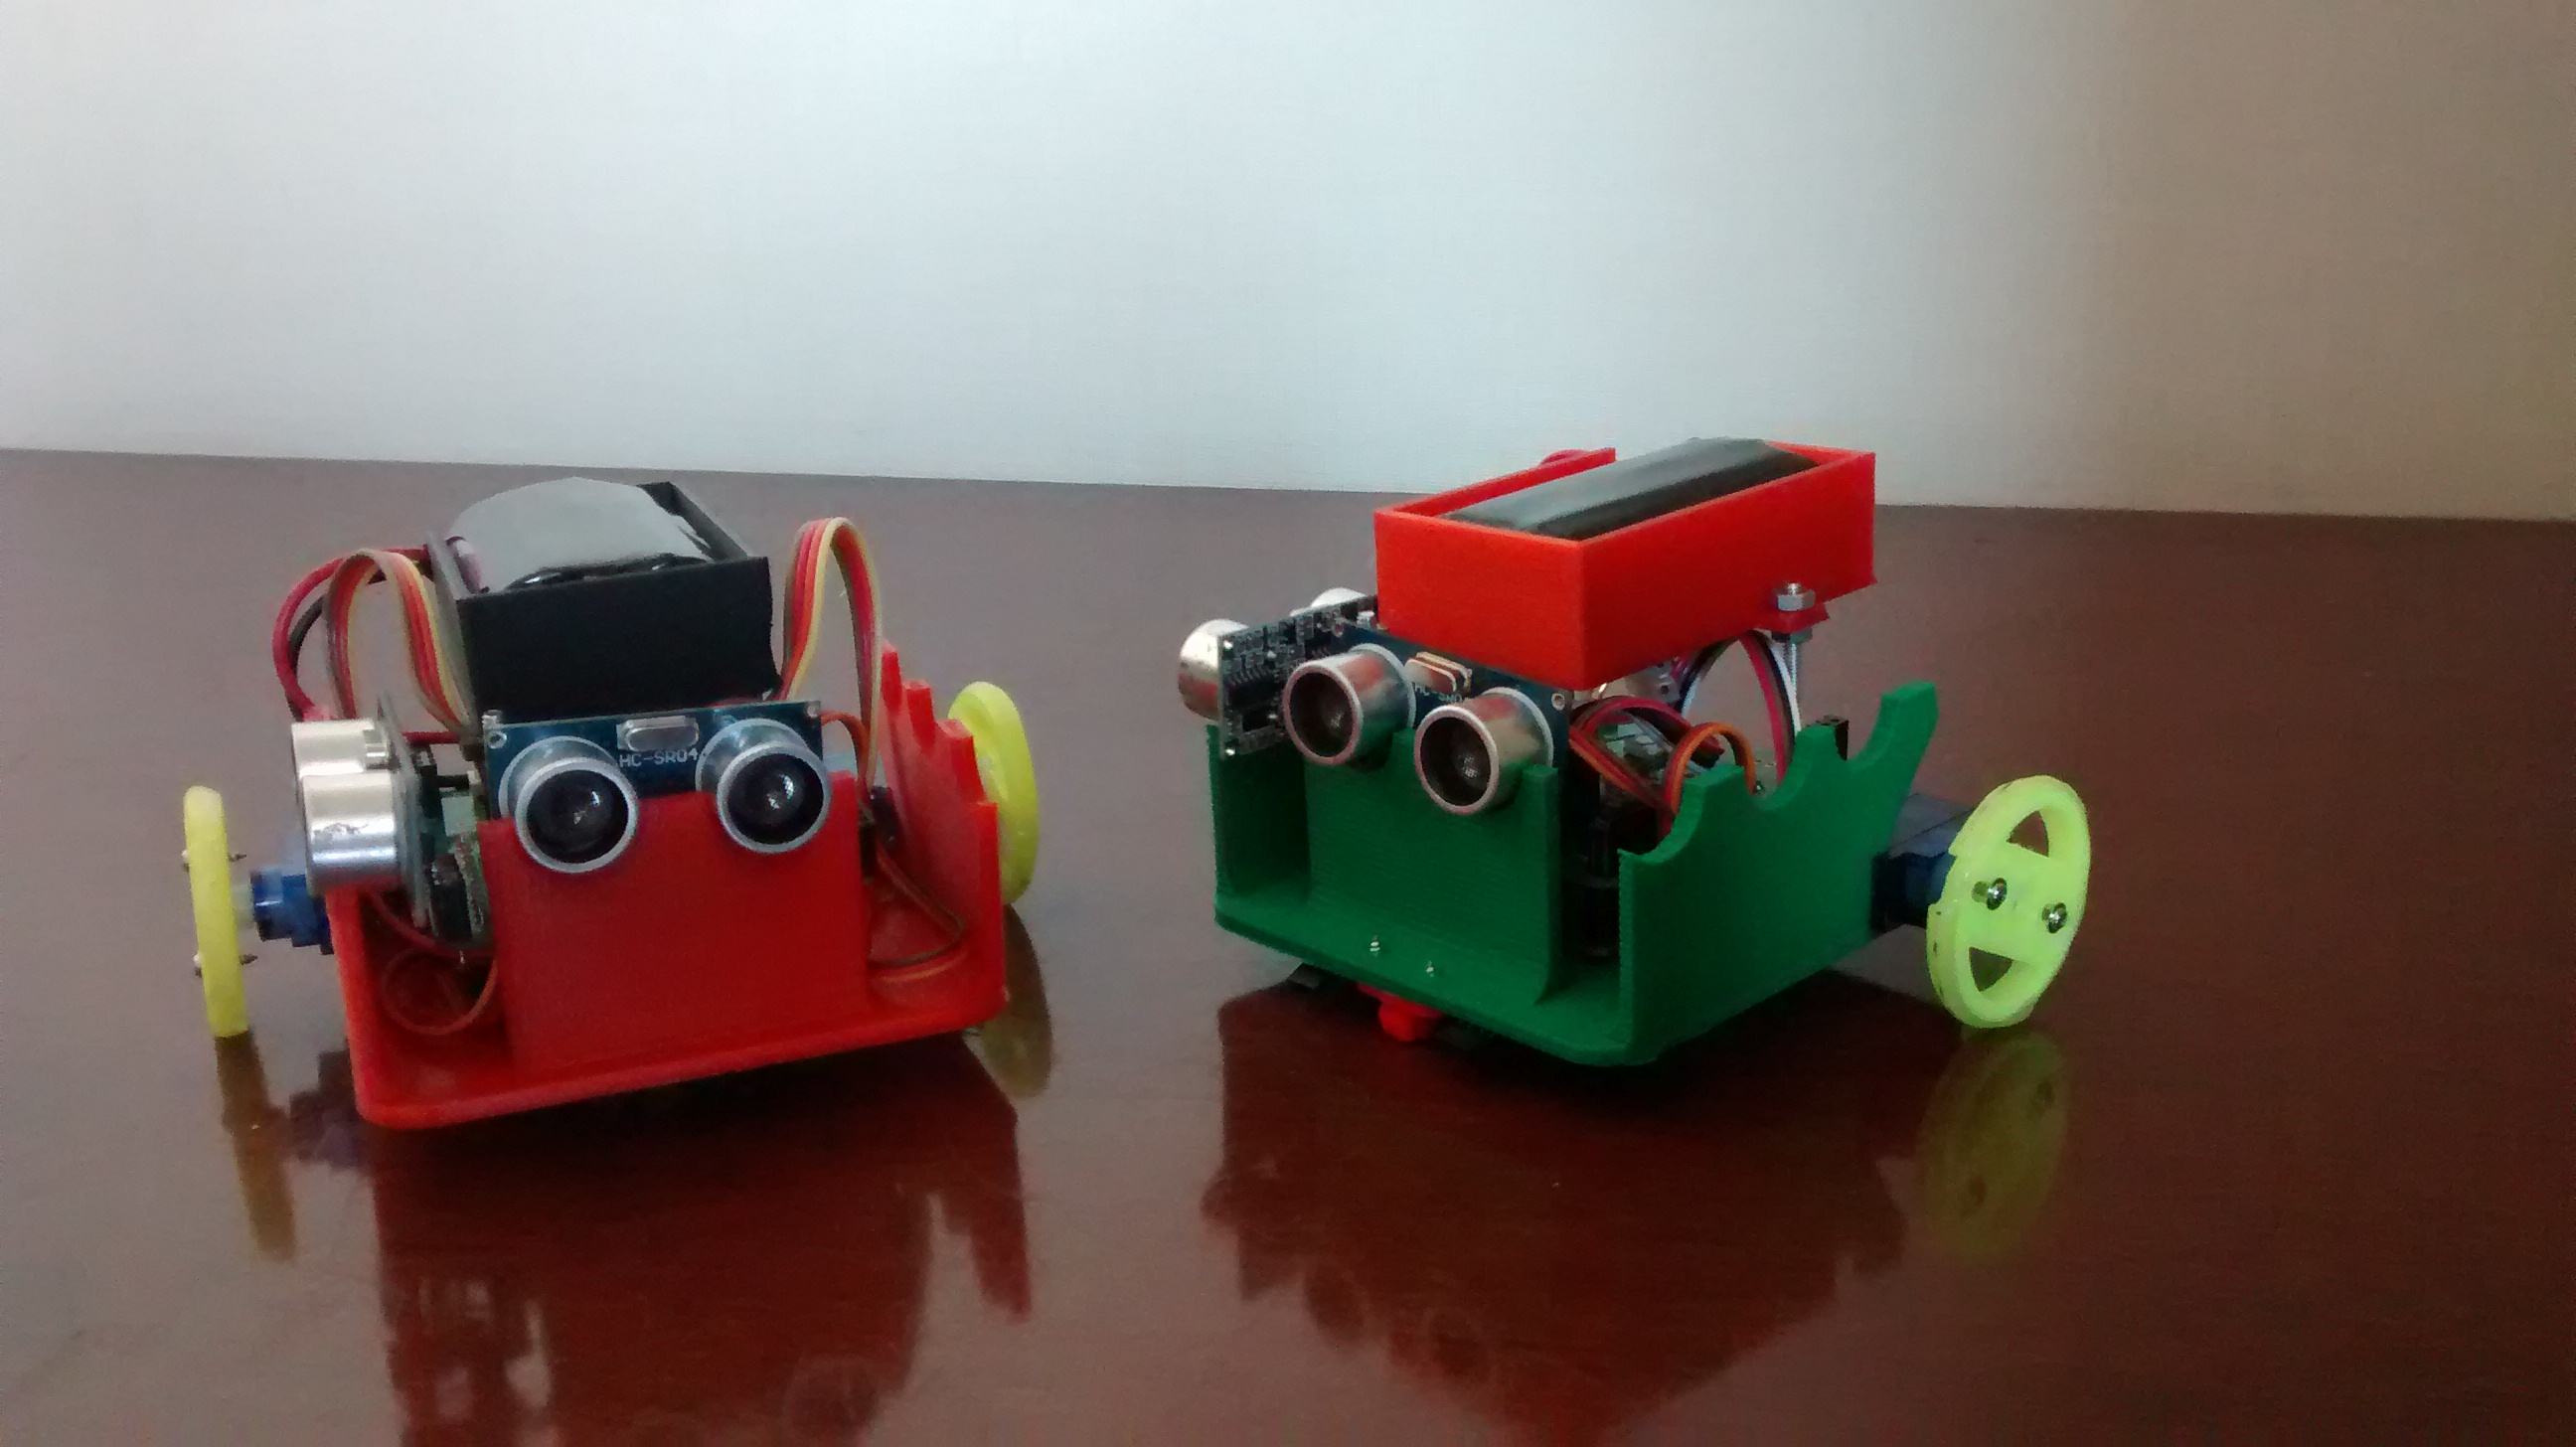
\includegraphics[height=0.8\textheight]{./img/dreamster-top.jpg} 
 \end{center}
\end{frame}

\begin{frame}
 \frametitle{El robot}
 \begin{center}
 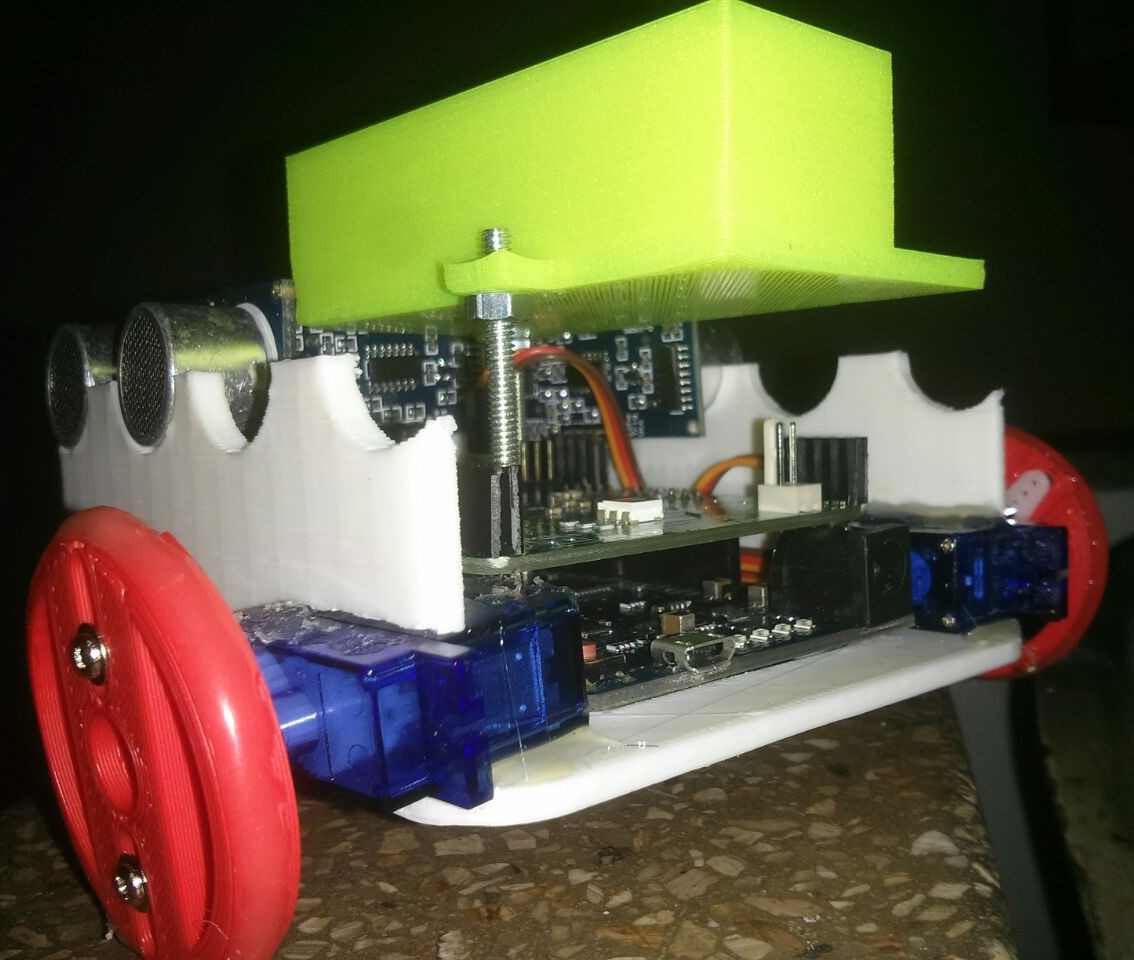
\includegraphics[height=0.8\textheight]{./img/dreamster-back.jpg} 
 \end{center}
\end{frame}

\section{Programación del Dreamster}
\subsection{Uso del compilador y IO}

\begin{frame}[fragile]
\frametitle{Nuestro primer código - Prender un led}

\begin{columns}
 \column{0.5\textwidth}
  \begin{Verbatim}[formatcom=\color{red},fontseries=b, numbers=left,numbersep=3pt]
  int led = 13;
  setup() {
    pinMode(led, OUTPUT);
  }
  loop() {
    digitalWrite(led, HIGH);
    delay(1000);
    digitalWrite(led, LOW);
    delay(1000);
  }
  \end{Verbatim} 
 \column{0.5\textwidth}

   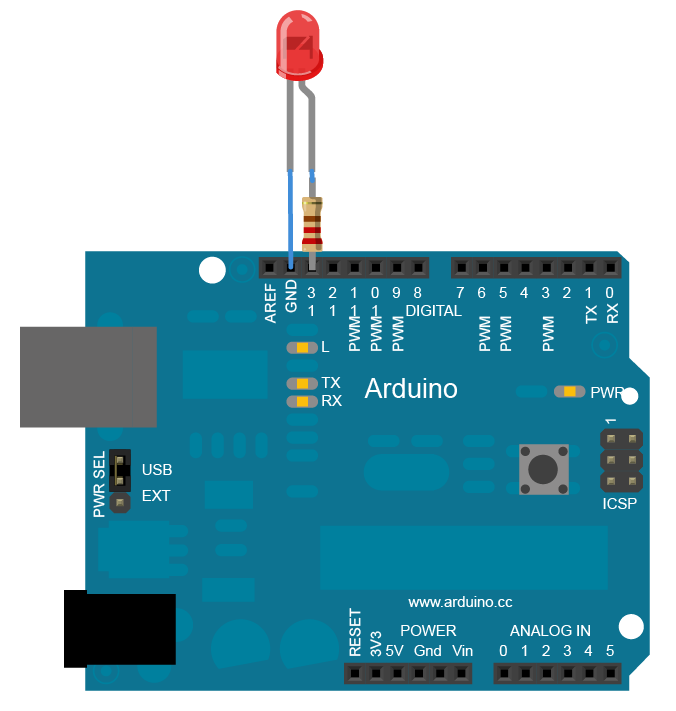
\includegraphics[width=\columnwidth]{./img/arduino_led.png}

\end{columns}


 \begin{center}
 \vspace{0.5cm}
 \textbf{Probemos si funciona!!!}
 \end{center}

\end{frame}

\subsection{Comunicarnos}
\begin{frame}[fragile]
 \frametitle{Puerte serie}

\begin{center}
 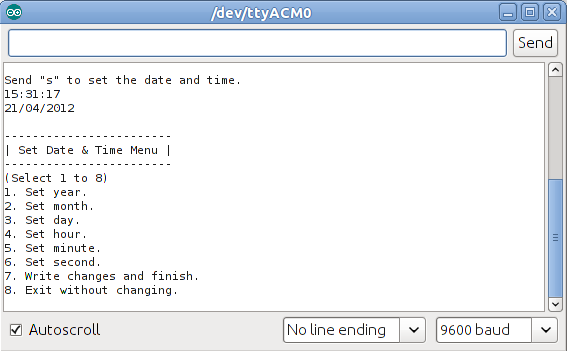
\includegraphics[height=0.4\textheight]{./img/serial.png}
\end{center}

\begin{Verbatim}[formatcom=\color{red},fontseries=b, numbers=left,numbersep=3pt,fontsize=\tiny]
int incomingByte = 0;

void setup() {
    // abre el puerto en 9600
    Serial.begin(9600);
}

void loop() {
    // Envio datos si me dicen algo por el serie
    if (Serial.available() > 0) {
        // leemos un byte:
        incomingByte = Serial.read();
        // devolvemos:
        Serial.print("Lei: ");
        Serial.println(incomingByte, DEC);
    }
}
\end{Verbatim}
\end{frame}

\subsection{Sensores de distancia}

\begin{frame}[fragile]
 \frametitle{Sensores de distancia - HC-SR04}
\begin{columns}
\column{0.7\textwidth}
Estos sensores nos permiten medir la distancia a un objeto mediante el uso de pulsos ultrasónicos.
\begin{center}
 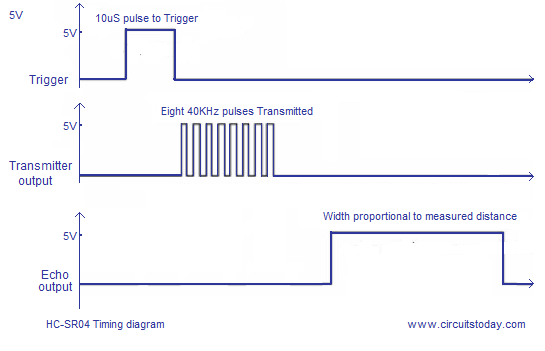
\includegraphics[width=1.0\columnwidth]{./img/hc-sr04-timing-diagram.png}
 % cny70.jpg: 250x238 pixel, 180dpi, 3.53x3.36 cm, bb=0 0 100 95
\end{center}
\column{0.3\textwidth}
\begin{center}
 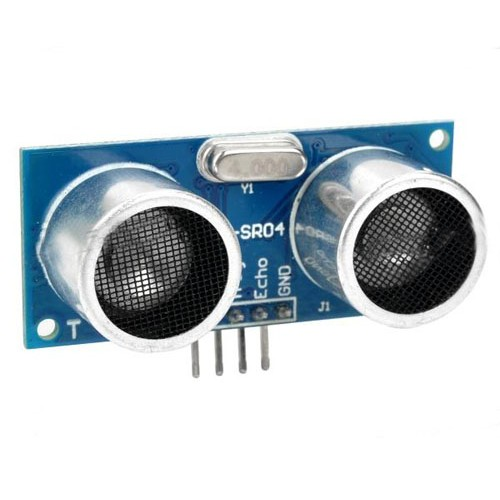
\includegraphics[width=1.0\columnwidth]{./img/hc-sr04.jpg}
 % sensor.pdf: 81x195 pixel, 72dpi, 2.86x6.88 cm, bb=0 0 81 195
\end{center}
\end{columns}
\end{frame}

\begin{frame}[fragile]
\frametitle{Usando el Sensor de distancia con Arduino}
\begin{columns}
 \column{0.5\textwidth}
  \begin{Verbatim}[formatcom=\color{red},fontseries=b, numbers=left,numbersep=3pt,fontsize=\tiny]
  const int TriggerPinA = A3;
  const int EchoPinA = 8;
  long Duration = 0;
  
  void setup(){
    pinMode(TriggerPinA, OUTPUT)
    pinMode(EchoPinA, INPUT);
    Serial.begin(9600);
  }
  
  void loop(){ 
    digitalWrite(TriggerPinA, LOW);                   
    delayMicroseconds(2);
    digitalWrite(TriggerPinA, HIGH);
    delayMicroseconds(10);
    digitalWrite(TriggerPinA, LOW);
   
    Duration = pulseIn(EchoPinA, HIGH);

    // Calculates the Distance in mm
    long Distance_mm = ((Duration /2.9) / 2);
   
    Serial.print("Distance = ");
    Serial.print(Distance_mm);
    Serial.println(" mm");
   
    delay(1000);
  }
    \end{Verbatim} 
 \column{0.5\textwidth}

   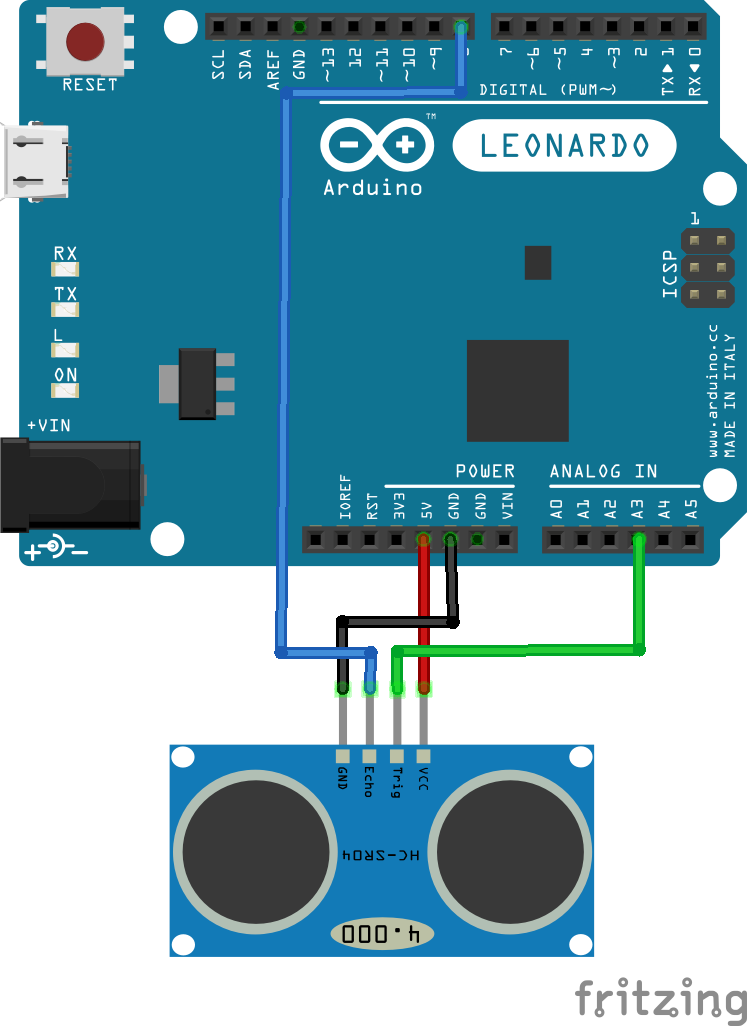
\includegraphics[width=\columnwidth]{./img/arduino_hc-sr04.png}

\end{columns}
\end{frame}

\subsection{Timers y PWM}

%\begin{frame}
% \frametitle{Intervalo!!}
%\vspace{2cm}
%\begin{center}
%\Huge{Nos vemos en 15 minutos.}
%\end{center}
%\vspace{2cm}
%\end{frame}

\section{Conociendo la planta}

\subsection{Actuadores y sensores}

\begin{frame}[fragile]
 \frametitle{Sensores - TCRT1000}
 \begin{columns}
\column{0.7\textwidth}

 \begin{Verbatim}[formatcom=\color{red},fontseries=b, numbers=left,numbersep=3pt]
const int sensor = A0;
const int led = 13;
...
// leer el valor del sensor
int medicion = analogRead(sensor);
// ajustamos el brillo del led
char out = map(medicion, 0, 1023, 0, 255);
analogWrite(led, out);
\end{Verbatim}

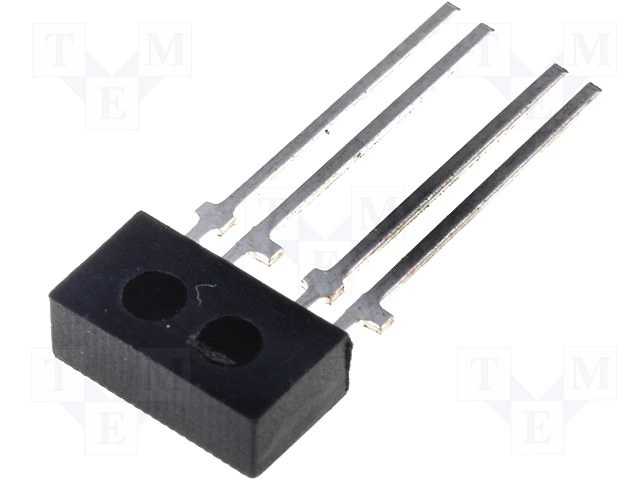
\includegraphics[width=0.3\columnwidth]{./img/tccrt1000.jpg}

\column{0.3\textwidth}
\begin{center}

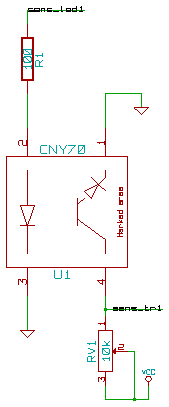
\includegraphics[width=0.8\columnwidth]{./img/sensor.pdf}
% sensor.pdf: 81x195 pixel, 72dpi, 2.86x6.88 cm, bb=0 0 81 195

\end{center}
\end{columns}
\end{frame}

\begin{frame}
\frametitle{Sensores - TCRT1000}
\begin{center}
 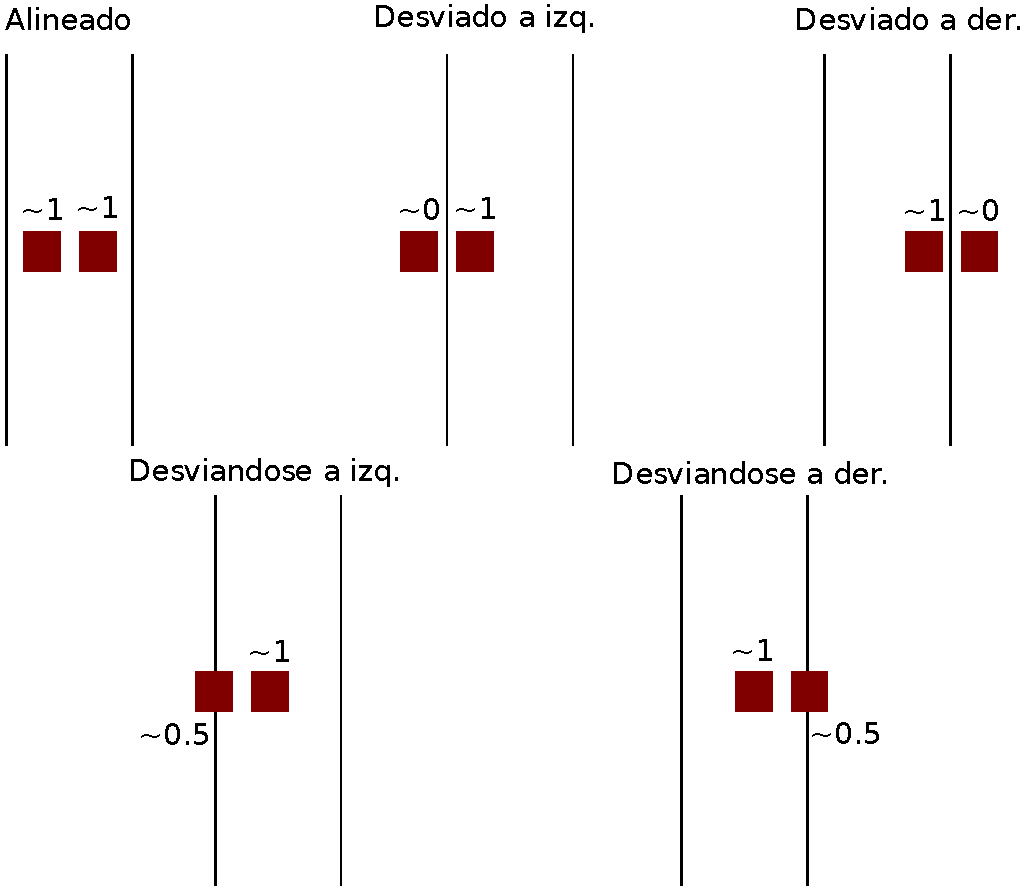
\includegraphics[height=0.8\textheight]{./img/sensores_image.pdf}
 % pwm_image.pdf: 166x91 pixel, 72dpi, 5.86x3.21 cm, bb=0 0 166 91
\end{center}
\end{frame}

\begin{frame}
 \frametitle{Puente H - DRV8833}
Para manejar los motores de CC usamos un IC (DRV8833) que tiene 2 puentes H.
\begin{columns}
\column{0.6\textwidth}
\begin{center}
 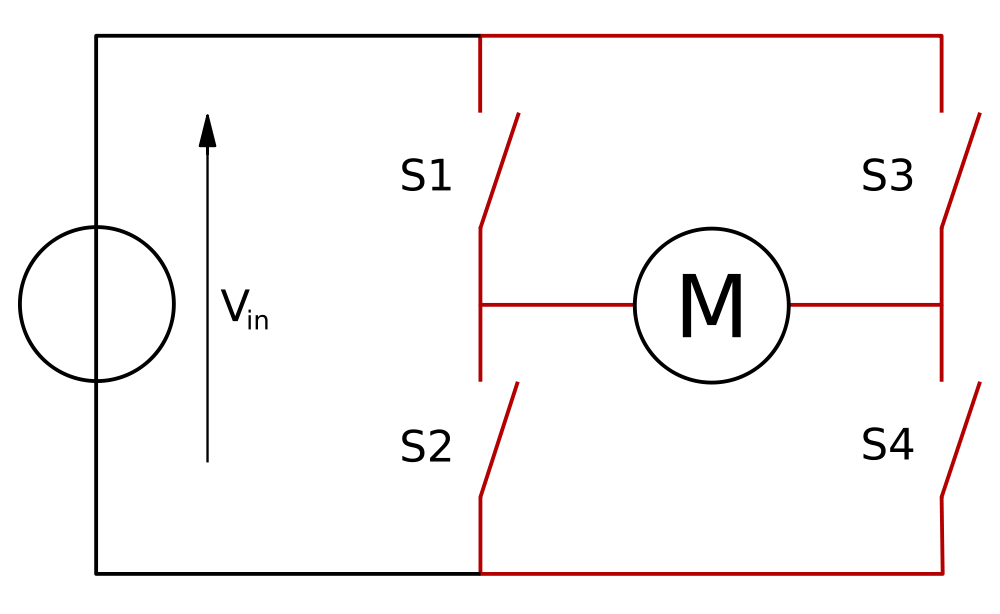
\includegraphics[width=\columnwidth]{./img/puenteH_1.png}
 % puenteH_1.png: 1000x614 pixel, 72dpi, 35.28x21.66 cm, bb=0 0 1000 614
\end{center}
\column{0.4\textwidth}
\begin{center}
 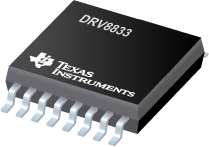
\includegraphics[width=\columnwidth]{./img/drv8833.jpg}
 % puenteH_1.png: 1000x614 pixel, 72dpi, 35.28x21.66 cm, bb=0 0 1000 614
\end{center}

\end{columns}
\end{frame}

\begin{frame}
 \frametitle{Puente H - DRV8833}
Con el puente H podemos cambiar el sentido y velocidad de los motores.
\begin{center}
 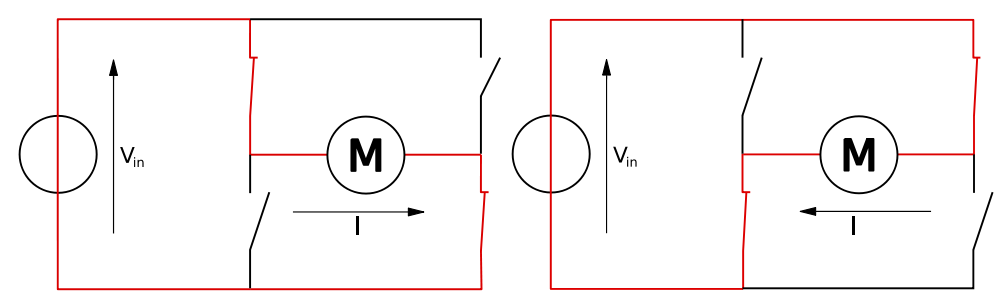
\includegraphics[width=\columnwidth]{./img/puenteH_2.png}
 % puenteH_1.png: 1000x614 pixel, 72dpi, 35.28x21.66 cm, bb=0 0 1000 614
\end{center}
.. y ¿Cómo variamos la velocidad?

\end{frame}

\begin{frame}
 \frametitle{Puente H - DRV8833}
\begin{columns} 
\column{0.4\textwidth}
{%
\begin{center}
\begin{tabular}{|c|c|c|}\hline
\textbf{IN1} & \textbf{IN2} & \textbf{Motor} \\ \hline
PWM & 0 & Adelante\\ \hline
0 & PWM & Atrás\\ \hline
1 & PWM & Adelante\\ \hline
PWM & 1 & Atrás\\ \hline
\end{tabular}
\end{center}
}%
\column{0.6\textwidth}
 \begin{center}
 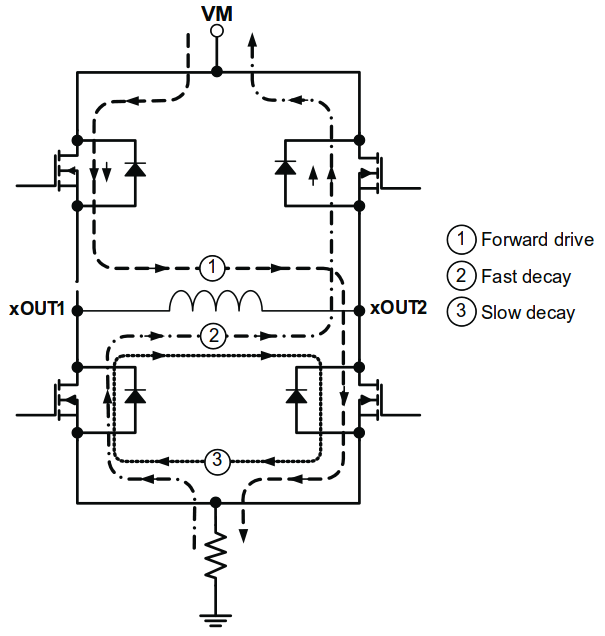
\includegraphics[width=\columnwidth]{./img/drv8833.png}
 % l298image.png: 322x353 pixel, 100dpi, 8.18x8.97 cm, bb=0 0 232 254
\end{center}
\end{columns}
\end{frame}

\begin{frame}[fragile]
 \frametitle{¿Pero que es un PWM?}
 \begin{columns}
 \column{0.4\textwidth}
\begin{Verbatim}[formatcom=\color{red},fontseries=b, numbers=left,numbersep=3pt, fontsize=\tiny]
int kMotorLP = 5;
int kMotorLN = 6;

/*
Configuramos los pines en cero para
apagar el motor
*/
void setup(){
  digitalWrite(kMotorLP, LOW);
  digitalWrite(kMotorLN, LOW);
}

void loop(){

  /*
  Incrementamos la velocidad progresivamente
  */
  digitalWrite(kMotorLN, LOW);
  for(int i = 0; i < 255; i++){
  	analogWrite(kMotorLP,  i);
  	delay(100);
  }

  /*
  Detenemos el motor para comenzar nuevamente
  */
  delay(1000);
  digitalWrite(kMotorLP, LOW);
  digitalWrite(kMotorLN, LOW);
  delay(1000);
}
\end{Verbatim}
  \column{0.55\textwidth}
  \flushright
  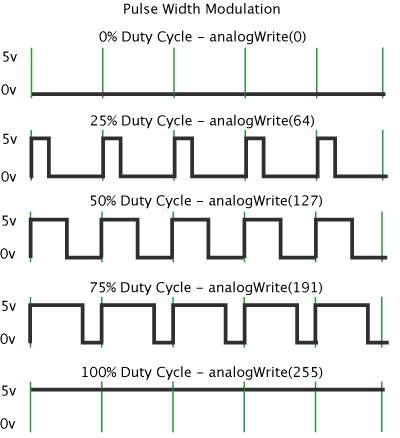
\includegraphics[width=\columnwidth]{./img/PWM.png}
 \end{columns}

\begin{center}
 
\end{center}
\end{frame}


\begin{frame}
\frametitle{A trabajar...}
Donde están conectadas las cosas en el Dreamster:
\begin{center}
\begin{tabular}{|c|c|c|c|}
\hline
\textbf{Función} & \textbf{PinName} & \textbf{Función} & \textbf{PinName}\\\hline
Motor Izq. P & 5 & Linea Izq. & A0\\\hline
Motor Izq. N & 6 & Linea Der. & A1\\\hline
Motor Der. P & 9 & Sensor US AT & A3\\\hline
Motor Der. N & 10 & Sensor US AE & 8\\\hline
Led Rojo & 12 & Sensor US BT & A4\\\hline
Led Verde & 11 & Sensor US BE & 2\\\hline
Led Azul & 13 & Sensor US CT & A5\\\hline
& & Sensor US CE & 7 \\\hline
\end{tabular}
\end{center}
\end{frame}

% La competencia
\begin{frame}
 \frametitle{La competencia}
Tareas:
\begin{itemize}
 \item Encontrar un objeto
 \item Moverse en la dirección del objeto
 \item Identificar el borde de la mesa
\end{itemize}
Qué podemos hacer:
\begin{itemize}
 \item Medir distancias
 \item Medir el color del piso
 \item Movernos
\end{itemize}
\end{frame}

\end{document}


